\documentclass{article}\usepackage[]{graphicx}\usepackage[]{color}
%% maxwidth is the original width if it is less than linewidth
%% otherwise use linewidth (to make sure the graphics do not exceed the margin)
\makeatletter
\def\maxwidth{ %
  \ifdim\Gin@nat@width>\linewidth
    \linewidth
  \else
    \Gin@nat@width
  \fi
}
\makeatother

\definecolor{fgcolor}{rgb}{0.345, 0.345, 0.345}
\newcommand{\hlnum}[1]{\textcolor[rgb]{0.686,0.059,0.569}{#1}}%
\newcommand{\hlstr}[1]{\textcolor[rgb]{0.192,0.494,0.8}{#1}}%
\newcommand{\hlcom}[1]{\textcolor[rgb]{0.678,0.584,0.686}{\textit{#1}}}%
\newcommand{\hlopt}[1]{\textcolor[rgb]{0,0,0}{#1}}%
\newcommand{\hlstd}[1]{\textcolor[rgb]{0.345,0.345,0.345}{#1}}%
\newcommand{\hlkwa}[1]{\textcolor[rgb]{0.161,0.373,0.58}{\textbf{#1}}}%
\newcommand{\hlkwb}[1]{\textcolor[rgb]{0.69,0.353,0.396}{#1}}%
\newcommand{\hlkwc}[1]{\textcolor[rgb]{0.333,0.667,0.333}{#1}}%
\newcommand{\hlkwd}[1]{\textcolor[rgb]{0.737,0.353,0.396}{\textbf{#1}}}%
\let\hlipl\hlkwb

\usepackage{framed}
\makeatletter
\newenvironment{kframe}{%
 \def\at@end@of@kframe{}%
 \ifinner\ifhmode%
  \def\at@end@of@kframe{\end{minipage}}%
  \begin{minipage}{\columnwidth}%
 \fi\fi%
 \def\FrameCommand##1{\hskip\@totalleftmargin \hskip-\fboxsep
 \colorbox{shadecolor}{##1}\hskip-\fboxsep
     % There is no \\@totalrightmargin, so:
     \hskip-\linewidth \hskip-\@totalleftmargin \hskip\columnwidth}%
 \MakeFramed {\advance\hsize-\width
   \@totalleftmargin\z@ \linewidth\hsize
   \@setminipage}}%
 {\par\unskip\endMakeFramed%
 \at@end@of@kframe}
\makeatother

\definecolor{shadecolor}{rgb}{.97, .97, .97}
\definecolor{messagecolor}{rgb}{0, 0, 0}
\definecolor{warningcolor}{rgb}{1, 0, 1}
\definecolor{errorcolor}{rgb}{1, 0, 0}
\newenvironment{knitrout}{}{} % an empty environment to be redefined in TeX

\usepackage{alltt}
\usepackage{enumerate}
\usepackage{enumitem}
\usepackage{lastpage}
\usepackage[margin=1in]{geometry}
\geometry{letterpaper}
\usepackage{rotating}
\usepackage{float}

\usepackage{amssymb,amsmath}
\usepackage{dsfont}
\usepackage{ifxetex,ifluatex}
\usepackage{fancyvrb}
\allowdisplaybreaks[1]
\usepackage{tabularx}

\newcommand{\expect}{\mathop{{}\mathbb{E}}}
\newcommand{\var}{\mathop{{}\mathbb{V}ar}}
\newcommand{\lik}[2]{\mathop{{}\mathcal{L}(#1 \vert #2)}}
\newcommand{\llik}[2]{\mathop{{}\ell(#1 \vert #2)}}
\newcommand{\deriv}[3]{\mathop{\frac{\delta^{#3}#1}{\delta #2^{#3}}}}
\newcommand{\crossderiv}[4]{\mathop{\frac{\delta^{#4}#1}{\delta #2 \, \delta #3}}}
\newcommand{\1}{\mathop{\mathds{1}}}

\newsavebox{\mybox}
\newenvironment{problem}
{\begin{lrbox}{\mybox}\begin{minipage}{0.9\textwidth}\bfseries}
{\end{minipage}\end{lrbox}\fbox{\rule[-20pt]{0pt}{40pt}\usebox{\mybox}}}

\newcommand\pline[1]{%
  \fbox{\parbox{\linewidth}{\textbf{#1}}}}
  
\title{CS 205: Homework 2}
\author{Eric Dunipace}
\date{March 22, 2017}
\IfFileExists{upquote.sty}{\usepackage{upquote}}{}
\begin{document}

\maketitle
\clearpage



\begin{enumerate}[label=\arabic*., start=2]
{\huge \item \textbf{Analysis of Parallel Algorithms [10\%]}}\\

\begin{enumerate}
  \item \pline{Define iso-efficiency function for an ideally scalable parallel system.}\\

Iso-efficiency for an ideally scalable parallel system measures how well we can maintain the same efficiency as we add processors to a given problem. As Manju says in lecture 5, iso-efficiency is ``the rate at which the problem size must increase with respect to the number of processing elements to keep the e ciency fixed.'' Put in another way, it is how easy it is to add processors to a given problem. Small iso-efficiency values indicate a problem is highly parallelizable; large iso-efficiency values indicate a problem is not highly parallelizable.\\

To derive this function, we start with efficiency, which equals \[E = \frac{S}{p},\] where $p$ is the number of processors and $S=\frac{T_1}{T_p}$ is the speedup achieved with $p$ processors. From here, \[S= \frac{Wp}{W + T_o(W,p)},\] where $W$ is the share of the serial work done on each parallel processor and $T_o(W,p)$ is the overhead of start-up and communication for the $p$ processors. Thus the work of one serial processor is simply $Wp$. Then, plugging back into efficiency, \[E = \frac{\frac{Wp}{W + T_o(W,p)}}{p} = \frac{W}{W + T_o(W,p)} = \frac{1}{1 + \frac{T_o(W,p)}{W}}.\] Solving for $W$ gives
  \begin{align*}
    E &= \frac{1}{1 + \frac{T_o(W,p)}{W}}\\
    E\left(1 + \frac{T_o(W,p)}{W} \right) &= 1\\
    E + E\frac{T_o(W,p)}{W} &= 1\\
    E\frac{T_o(W,p)}{W} &= 1-E\\
    \frac{E T_o(W,p)}{1-E} &= W,\\
    \intertext{then taking $\frac{E}{1-E}$ as a constant $K$ of the desired efficiency}
    W &= K T_o(W,p)\\
  \end{align*}
  



 \item \pline{Scaled speed-up is defined as the speedup obtained when the problem size is increased linearly with the number of processing elements; that is, if $W$ is chosen as a base problem size for a single processing element, then \[\text{scaled speedup} = \frac{pW}{T_p(pW, p)}.\] For the problem of adding $n$ numbers on $p$ processing elements, assume that it takes 20 time units to communicate a 
number between two processing elements, and that it takes one unit of time to add two numbers. Plot the 
standard speedup curve for the base problem size $p = 1, n = 256$ and compare it with the scaled speedup 
curve with $p = 2^2, 2^4, 2^5, 2^8$.}
 
 Assuming that $T_p(pW, p)$ is the standard parallel time to run the algorithm, then the following code calculates the scaled speed up versus the standard speedup calculations.\\
\begin{knitrout}
\definecolor{shadecolor}{rgb}{0.969, 0.969, 0.969}\color{fgcolor}\begin{kframe}
\begin{alltt}
import numpy as np
import matplotlib.pyplot as plt
import math
import matplotlib.patches as mpatches

#processors
exponents  = [2,4,5,8]
p = [2**i for i in exponents]

#problem size
n = 2**8 #256

#costs
comm = 20
W_t = 1 # work per time to sum 2 numbers

def serial_time(w_t, n):
   T_1 = n*w_t
   return(T_1)

def parallel_time(p, C, w_t, n):    
   T_p = serial_time(w_t,n/p) + C
   for i in range(p):
       T_p += C + p/(2**i)*w_t
   return(T_p)

def standard_speed(p, C, w_t, n):
   T_p = parallel_time(p, C, w_t, n)
   T_1 = serial_time(w_t, n)
   
   return(T_1/T_p)

def scaled_speedNoComm(p, w_t, n):
   T_p = serial_time(w_t, n / p)
   T_s = 0
   
   total = T_s + T_p * p

   return(p - (p - 1) * (T_s / total))

def scaled_speed(p, C, w_t, n):
   T_p = serial_time(w_t, n/p) + C
   T_s = 0
   for i in range(p):
       T_s += C + p/(2**i)*w_t
   
   total = T_s + T_p * p
   return(p - (p - 1) * T_s/total)
   #return((T_s / total) + p * (1 - T_s / total))



scale = [scaled_speed(i,comm, W_t, n) for i in p]
scaleNoCom = [scaled_speedNoComm(i, W_t, n) for i in p]
stand = [standard_speed(i, comm, W_t, n) for i in p]
axes = plt.gca()
plt.figure(1)
plt.plot(p, stand, '-b', label='Standard Speed-up')
plt.plot(p, scale, '-r', label='Scaled Speed-up (With Communication)')
plt.plot(p, scaleNoCom, '-k', label='Scaled Speed-up (No Communication)')
axes.set_ylim([0,np.ceil(max(scale + stand + scaleNoCom))+1])
axes.set_xlim([0,max(p)])
plt.xlabel('Number of Processors')
plt.ylabel('Speed-up')
plt.title('Plot of Speed-up Versus Time')
plt.legend(loc=2)
plt.savefig("figures/speedup.png")

plt.figure(3)
axes = plt.gca()
plt.plot(p, stand, '-b', label='Standard Speed-up')
axes.set_ylim([0,np.ceil(max(stand ))])
axes.set_xlim([0,max(p)])
# plt.yscale('log')
plt.xlabel('Number of Processors')
plt.ylabel('Speed-up')
plt.title('Plot of Stand Speed-up Versus Time')
plt.savefig("figures/speedup2.png")

\end{alltt}
\end{kframe}
\end{knitrout}
\begin{figure}[H]
  \centering
    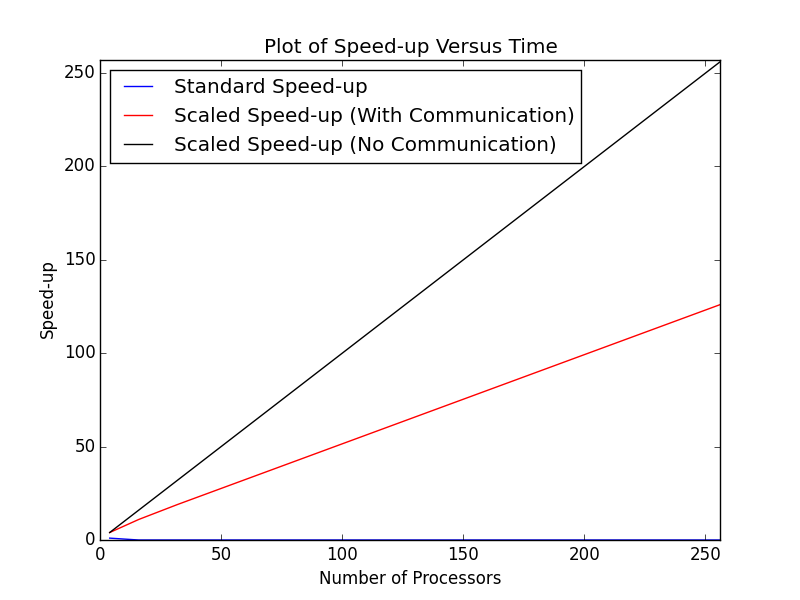
\includegraphics[width=0.4\textwidth]{figures/speedup.png}
    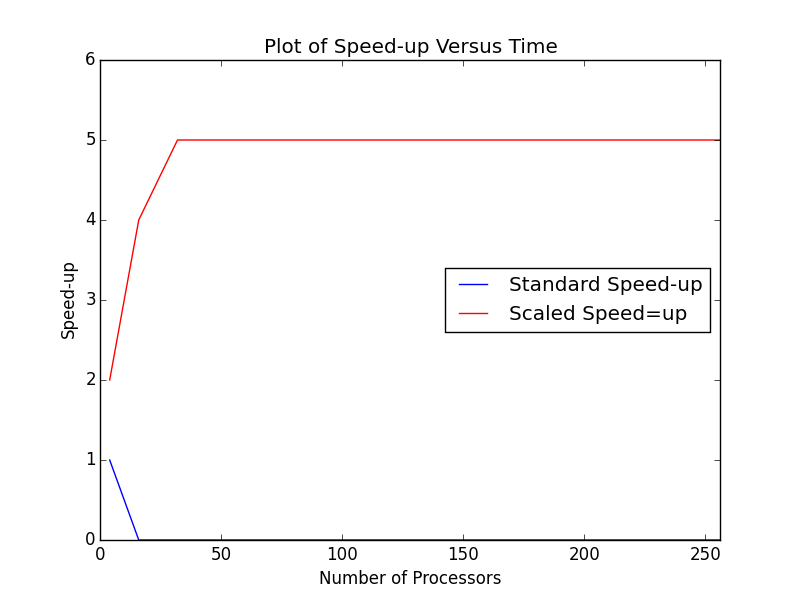
\includegraphics[width=0.4\textwidth]{figures/speedup2.png}
    \caption{Comparison of standard speed-up versus scaled speed-up, where scaled speed-up increases the base problem size of $n=256$ elements by a factor of the processors, $p$. Close up of standard speed up presented to actually see the line}

  \end{figure}
\end{enumerate}

{\huge \item \textbf{Parallel Matrix Algorithms in CUDA and OpenAcc [40\%]}}

In this problem we will revisit the tiling transformation from HW1 and investigate parallel algorithm design and implementation
for Matrix Multiplication in the SIMT programming model for Manycore GPU architecture.\\

We have studied two ways to construct parallel programs for GPU architectures. CUDA programs use explicit parallel programming
to express parallelism and to specify locality. OpenAcc, in contrast, provides a directive based mechanism to implement parallel
programs through an automatic compilation system that generates parallel programs from annotated sequential programs. This offers a 
programming approach to rapidly implement different versions of parallel programs which simplifies the task of exploring the solution 
space for an efficient parallel program.\\

In this programming task you will implement and optimize the tiled Matrix Multiplication in the two programming languages as follows:\\

\begin{enumerate}[label=\arabic*.]
\item \pline{CUDA}

 \begin{enumerate}[label=(\alph*)]
    \item \pline{First benchmark a naive version (nested three loop matrix multiplication CUDA parallel program) against the reference implementation in CUBLAS. Generate a performance plot of throughput (GFlop/s) for problem sizes $n = 2^6, 2^{10}, 2^{16}$ for single precision floating point real numbers and compare against CUBLAS.}\\
  
  \item \pline{Implement a tiled parallel matrix multiplication program using the same relationship as before: make the block size $b$ as large as possible so that $3b^2 \leq M$, where $M$ is the size of the "fast" memory on a GPU node.}
  
  \item \pline{Benchmark for problem sizes $n = 2^6, 2^{10}, 2^{16}.$}
  \end{enumerate}
  
\item \pline{OpenAcc}
  \begin{enumerate}[label=(\alph*)]
    \item \pline{Implement a tiled parallel matrix multiplication using gang (thread blocks), vector (threads) and tile features for loop scheduling and optimization.}\\
  
    \item \pline{Tune the performance by varying gang, vector and tile parameters. Carefully consider the vector size in relation to warp size.}
  
    \item \pline{Benchmark for problem sizes $n = 2^6, 2^{10}, 2^{16}.$}
  
    \item \pline{What is the search space of the above brute force approach for very large problem size $n$? Is there a better way to search the space of parallel programs in (b) than brute force? Briefly discuss in the write-up.}
    \end{enumerate}
  
\end{enumerate}
\end{enumerate}

Submission: A write-up covering the following aspects uploaded as a single PDF file.
  \begin{itemize}
   \item A short one page description of the diffrent design principles that was used to develop successive versions of the parallel program.
   \item The optimizations used and the results obtained with reference to performane plots.
   \item Code listing and test cases (runs from single vs parallel to validate correctness of outputs).
   \item Performance plots of throughput (GFlop/s). The plot should indicate the peak throughput achievable on the GPU node and should compare the two versions of the implementations.
  \end{itemize}



\end{document}
